The BVH file format was originally developed by Biovision, a motion capture services company, as a way to provide motion capture data to their customers. The name BVH stands for Biovision hierarchical data. This format mostly replaced an earlier format that they developed, the BVA format, as a way to provide skeleton hierarchy information in addition to the motion data. The BVH format is an excellent all-around format, its only drawback is the lack of a full definition of the basis pose (this format has only translational offsets of children segments from their parent, no rotational offset is defined), it also lacks explicit information for how to draw the segments but that has no bearing on the definition of the motion.\\

A BVH file has two parts, a header section that describes the hierarchy and initial pose of the skeleton; and a data section that contains the motion data. The start of the header section begins with the keyword "HIERARCHY". The following line starts with the keyword "ROOT" followed by the name of the root segment of the hierarchy to be defined. After this hierarchy is described it is permissible to define another hierarchy, this too would be denoted by the keyword "ROOT". In principle, a BVH file may contain any number of skeleton hierarchies. In practice the number of segments is limited by the format of the motion section, one sample in time for all segments is on one line of data and this will cause problems for readers which assume a limit to the size of a line in a file.\\

The BVH format now becomes a recursive definition. Each segment of the hierarchy contains some data relevant to just that segment then it recursively defines its children. The line following the ROOT keyword contains a single left curly brace '\{', the brace is lined up with the "ROOT" keyword. The line following a curly brace is indented by one tab character, these indentations are mostly to just make the file more human-readable but some BVH file parsers expect the tabs. The first piece of information about a segment is the offset of that segment from its parent, or in the case of the root object, the offset will generally be zero. The offset is specified by the keyword "OFFSET" followed by the X, Y, and Z offset of the segment from its parent. The offset information also indicates the length and direction used for drawing the parent segment. In the BVH format, there isn't any explicit information about how a segment should be drawn. This is usually inferred from the offset of the first child defined for the parent. Typically, only the root and the upper body segments will have multiple children.\\

The line following the offset contains the channel header information. This has the "CHANNELS" keyword followed by a number indicating the number of channels and then a list of that many labels indicating the type of each channel. The BVH file reader must keep track of the channel count and the types of channels encountered as the hierarchy information is parsed. Later, when the motion information is parsed, this ordering will be needed to parse each line of motion data. This format appears to have the flexibility to allow for segments that have any number of channels that can appear in any order.\\

You can see that the order of the rotation channels appears a bit odd, it goes Z rotation, followed by the X rotation, and finally the Y rotation. On the line of data following the specification of the channel, there can be one of two keywords, either you will find the "JOINT" keyword or you will see the "End Site" keyword. A joint definition is identical to the root definition except for the number of channels. This is where the recursion takes place, the rest of the parsing of the joint information proceeds just like a root. The end site information ends the recursion and indicates that the current segment is an end effector (has no children). The end site definition provides one more bit of information, it gives the length of the preceding segment just like the offset of a child defines the length and direction of its parent's segment. The end of any joint, end site, or root definition is denoted by a right curly brace '\}'. This curly brace is lined up with its corresponding right curly brace.\\

The motion section begins with the keyword "MOTION" on a line by itself. This line is followed by a line indicating the number of frames, this line uses the "Frames:" keyword (the colon is part of the keyword) and a number indicating the number of frames, or motion samples that are in the file. On the line after the frame definition is the "Frame Time:" definition, this indicates the sampling rate of the data. The rest of the file contains the actual motion data. Each line is one sample of motion data. The numbers appear in the order of the channel specifications as the skeleton hierarchy was parsed. In the figure below, we can see the hierarchy as well as the motion format of our Skeleton that we discussed in this section.

\pagebreak

\begin{figure}[htp]
    \centering
    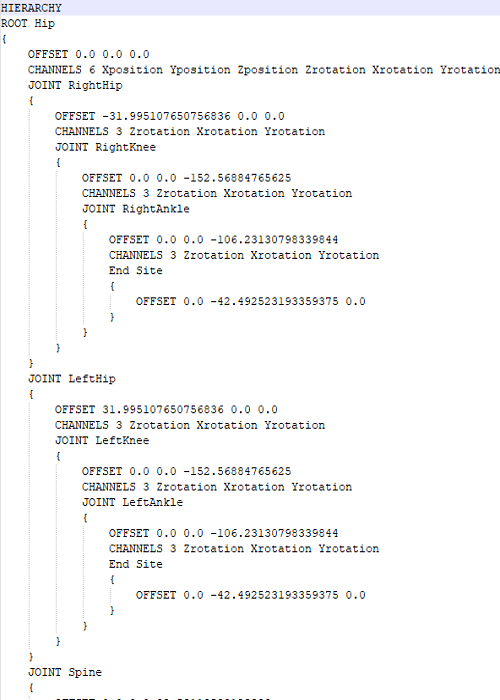
\includegraphics[width=7.5cm]{figures/Implementation/bvh1.png}%
    \qquad
    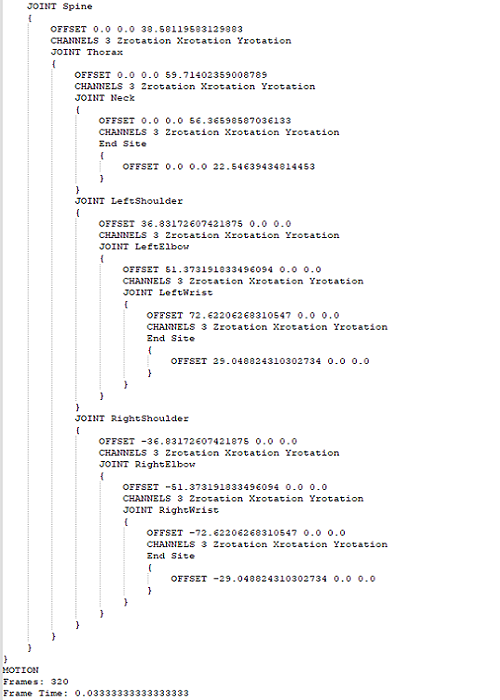
\includegraphics[width=7.5cm]{figures/Implementation/bvh2.png}%
    \qquad
    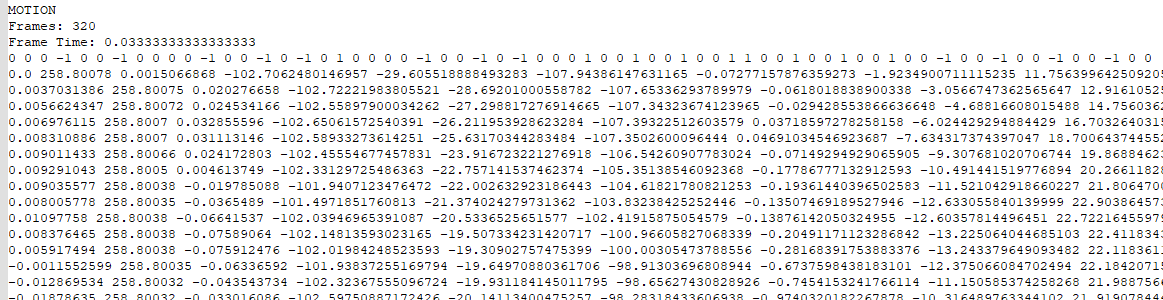
\includegraphics[width=1\textwidth]{figures/Implementation/bvh3.png}%
    \captionsetup{labelformat=empty}
    \caption{BVH format of the motion and hierarchy for the Skeleton that we are using. The first line of the motion, sets the skeleton in T-Pose and the rest contain the motion data.}
\end{figure}

